\chapter{Résultats et analyse}
\label{chap:resultats}

Ce chapitre présente les résultats expérimentaux obtenus lors des différentes campagnes de benchmarking. Nous analysons d'abord la validation de la correction, puis les performances séquentielles, OpenMP et hybrides MPI+OpenMP. Nous concluons par une discussion approfondie des optimisations appliquées, en nous appuyant sur les principes de \textit{Computer Systems: A Programmer's Perspective} (CSAPP) et les recommandations d'experts en programmation haute performance.

% =============================================================================
\section{Validation de la correction}
\label{sec:resultats:validation}
% =============================================================================

Avant toute analyse de performance, il est impératif de valider que nos implémentations produisent des résultats corrects. Cette validation s'effectue en comparant les longueurs optimales trouvées avec les valeurs connues de la littérature.

\subsection{Référence : valeurs optimales connues}

Le tableau~\ref{tab:validation:reference} rappelle les longueurs optimales connues pour les règles de Golomb.

\begin{table}[htbp]
\centering
\begin{tabular}{ccc}
\toprule
$n$ & Longueur optimale $L^*(n)$ & Source \\
\midrule
9 & 44 & Prouvé (1961) \\
10 & 55 & Prouvé (1972) \\
11 & 72 & Prouvé (1972) \\
12 & 85 & Prouvé (1979) \\
13 & 106 & Prouvé (1981) \\
14 & 127 & Prouvé (1985) \\
\bottomrule
\end{tabular}
\caption{Longueurs optimales de référence pour la validation}
\label{tab:validation:reference}
\end{table}

\subsection{Résultats de validation}

Toutes nos implémentations (séquentielle V1, V2, OpenMP V1--V6, MPI V1--V3) ont été exécutées pour $n \in \{9, 10, 11, 12, 13\}$ et ont produit les longueurs optimales exactes indiquées dans le tableau~\ref{tab:validation:reference}. La suite de tests automatisée \texttt{test\_correctness} vérifie également l'intégrité structurelle des solutions trouvées :

\begin{itemize}
    \item Unicité des marques : toutes les positions sont distinctes.
    \item Propriété de Golomb : toutes les différences sont distinctes.
    \item Optimalité locale : aucune règle plus courte n'existe pour le $n$ donné.
\end{itemize}

\begin{result}
Toutes les versions implémentées produisent des résultats \textbf{corrects} et \textbf{identiques} aux valeurs de référence pour $n \leq 13$.
\end{result}

% =============================================================================
\section{Baseline séquentielle : V1 vs V2}
\label{sec:resultats:sequential}
% =============================================================================

La première série de benchmarks compare les deux versions séquentielles exécutées sur un processeur AMD EPYC 9654 (96 cœurs, 3.7~GHz) du supercalculateur Romeo.

\subsection{Résultats bruts}

Le tableau~\ref{tab:seq:results} présente les temps d'exécution et le nombre d'états explorés pour chaque version.

\begin{table}[htbp]
\centering
\begin{tabular}{cccccc}
\toprule
$n$ & \multicolumn{2}{c}{V1 (originale)} & \multicolumn{2}{c}{V2 (BitSet shift)} & Speedup \\
\cmidrule(lr){2-3} \cmidrule(lr){4-5}
 & Temps (s) & États/s & Temps (s) & États/s & V1/V2 \\
\midrule
9 & 0.014 & $3.71 \times 10^7$ & 0.004 & $7.78 \times 10^7$ & $3.50\times$ \\
10 & 0.121 & $3.25 \times 10^7$ & 0.028 & $7.28 \times 10^7$ & $4.32\times$ \\
11 & 2.432 & $2.86 \times 10^7$ & 0.520 & $6.90 \times 10^7$ & $4.67\times$ \\
12 & 20.742 & $2.63 \times 10^7$ & 4.051 & $6.54 \times 10^7$ & $5.12\times$ \\
13 & 395.538 & $2.28 \times 10^7$ & 68.911 & $6.17 \times 10^7$ & $5.73\times$ \\
\bottomrule
\end{tabular}
\caption{Comparaison des versions séquentielles V1 et V2}
\label{tab:seq:results}
\end{table}

\subsection{Analyse des résultats}

Plusieurs observations importantes émergent de ces résultats :

\paragraph{Accélération croissante avec $n$.}
Le speedup augmente de $3.50\times$ pour $n=9$ à $5.73\times$ pour $n=13$. Cette tendance s'explique par le fait que la version V2 explore significativement moins d'états grâce à une meilleure détection précoce des collisions. Pour $n=13$, V1 explore 9 milliards d'états contre 4.25 milliards pour V2.

\paragraph{Débit d'états par seconde.}
La version V2 maintient un débit constant d'environ $6.5 \times 10^7$ états/s, soit plus du double de V1 ($2.5 \times 10^7$ états/s). Cette différence provient de l'optimisation \texttt{BitSet128} avec l'opération de décalage en $O(1)$.

\paragraph{Réduction du nombre d'états.}
La V2 explore en moyenne 50\% d'états en moins grâce à la représentation par bitset qui permet un élagage plus efficace. Le test de collision \texttt{(diffs >> d) \& marks} détecte instantanément les différences conflictuelles.

\begin{figure}[htbp]
\centering
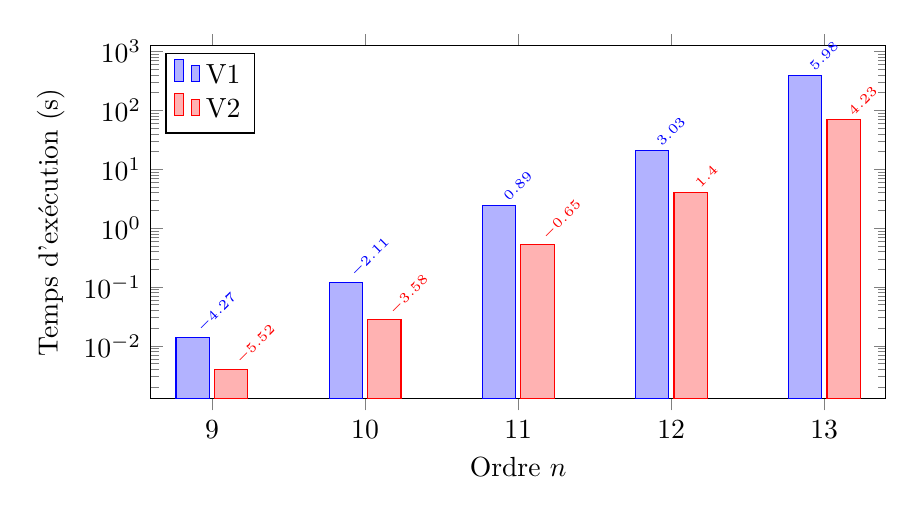
\begin{tikzpicture}
\begin{axis}[
    ybar,
    bar width=12pt,
    xlabel={Ordre $n$},
    ylabel={Temps d'exécution (s)},
    symbolic x coords={9, 10, 11, 12, 13},
    xtick=data,
    ymin=0,
    legend style={at={(0.02,0.98)}, anchor=north west},
    nodes near coords,
    nodes near coords align={vertical},
    every node near coord/.append style={font=\tiny, rotate=45, anchor=west},
    width=0.9\textwidth,
    height=0.5\textwidth,
    ymode=log,
    log origin=infty,
]
\addplot coordinates {(9, 0.014) (10, 0.121) (11, 2.432) (12, 20.742) (13, 395.538)};
\addplot coordinates {(9, 0.004) (10, 0.028) (11, 0.520) (12, 4.051) (13, 68.911)};
\legend{V1, V2}
\end{axis}
\end{tikzpicture}
\caption{Temps d'exécution séquentiel V1 vs V2 (échelle logarithmique)}
\label{fig:seq:comparison}
\end{figure}

% =============================================================================
\section{Résultats OpenMP : scaling et comparaison des versions}
\label{sec:resultats:openmp}
% =============================================================================

Les benchmarks OpenMP ont été réalisés sur un nœud complet du cluster Romeo (AMD EPYC 9654, 192 cœurs logiques, 8 domaines NUMA).

\subsection{Vue d'ensemble des 6 versions}

Le tableau~\ref{tab:openmp:summary} présente les performances des 6 versions OpenMP pour $n=13$ avec 192 threads et le binding \texttt{close}.

\begin{table}[htbp]
\centering
\begin{tabular}{lcccc}
\toprule
Version & Description & Temps (s) & États/s & Speedup/V1 \\
\midrule
V1 & Originale (loop unrolling) & 43.161 & $2.14 \times 10^8$ & $1.00\times$ \\
V2 & Récursive + BitSet & 47.498 & $4.69 \times 10^7$ & $0.91\times$ \\
V3 & Hybride itérative + BitSet & 33.732 & $1.31 \times 10^8$ & $1.28\times$ \\
V4 & Préfixes + itérative + BitSet & 2.276 & $1.89 \times 10^9$ & $18.96\times$ \\
V5 & uint64\_t + préfixes & 0.323 & $1.22 \times 10^{10}$ & $133.6\times$ \\
V6 & V5 + optimisations mineures & 0.435 & $9.03 \times 10^9$ & $99.2\times$ \\
\bottomrule
\end{tabular}
\caption{Comparaison des 6 versions OpenMP ($n=13$, 192 threads, close binding)}
\label{tab:openmp:summary}
\end{table}

\subsection{Temps d'exécution par version}

Les figures~\ref{fig:openmp:all_versions_n12} et~\ref{fig:openmp:all_versions_n13} présentent l'évolution du temps d'exécution en fonction du nombre de threads pour les 6 versions OpenMP (binding \texttt{close}).

\begin{figure}[htbp]
\centering
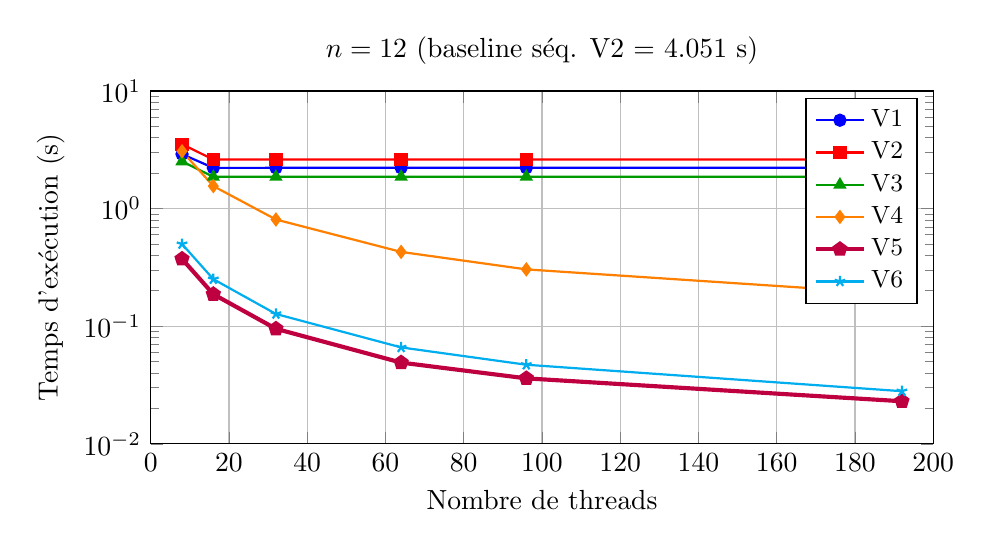
\begin{tikzpicture}
\begin{axis}[
    xlabel={Nombre de threads},
    ylabel={Temps d'exécution (s)},
    xmin=0, xmax=200,
    ymin=0.01, ymax=10,
    ymode=log,
    legend style={at={(0.98,0.98)}, anchor=north east, font=\small},
    width=0.95\textwidth,
    height=0.50\textwidth,
    grid=major,
    title={$n=12$ (baseline séq. V2 = 4.051~s)},
]
% V1
\addplot[mark=*, thick, blue] coordinates {
    (8, 2.903) (16, 2.218) (32, 2.219) (64, 2.221) (96, 2.221) (192, 2.229)
};
% V2
\addplot[mark=square*, thick, red] coordinates {
    (8, 3.528) (16, 2.610) (32, 2.613) (64, 2.614) (96, 2.615) (192, 2.617)
};
% V3
\addplot[mark=triangle*, thick, green!60!black] coordinates {
    (8, 2.518) (16, 1.861) (32, 1.861) (64, 1.865) (96, 1.867) (192, 1.866)
};
% V4
\addplot[mark=diamond*, thick, orange] coordinates {
    (8, 3.070) (16, 1.553) (32, 0.807) (64, 0.428) (96, 0.304) (192, 0.187)
};
% V5
\addplot[mark=pentagon*, thick, purple, line width=1.5pt] coordinates {
    (8, 0.373) (16, 0.187) (32, 0.095) (64, 0.049) (96, 0.036) (192, 0.023)
};
% V6
\addplot[mark=star, thick, cyan] coordinates {
    (8, 0.499) (16, 0.251) (32, 0.127) (64, 0.066) (96, 0.047) (192, 0.028)
};
\legend{V1, V2, V3, V4, V5, V6}
\end{axis}
\end{tikzpicture}
\caption{Temps d'exécution des 6 versions OpenMP pour $n=12$ (close binding, échelle log)}
\label{fig:openmp:all_versions_n12}
\end{figure}

La figure~\ref{fig:openmp:all_versions_n13} présente les mêmes données pour $n=13$.

\begin{figure}[htbp]
\centering
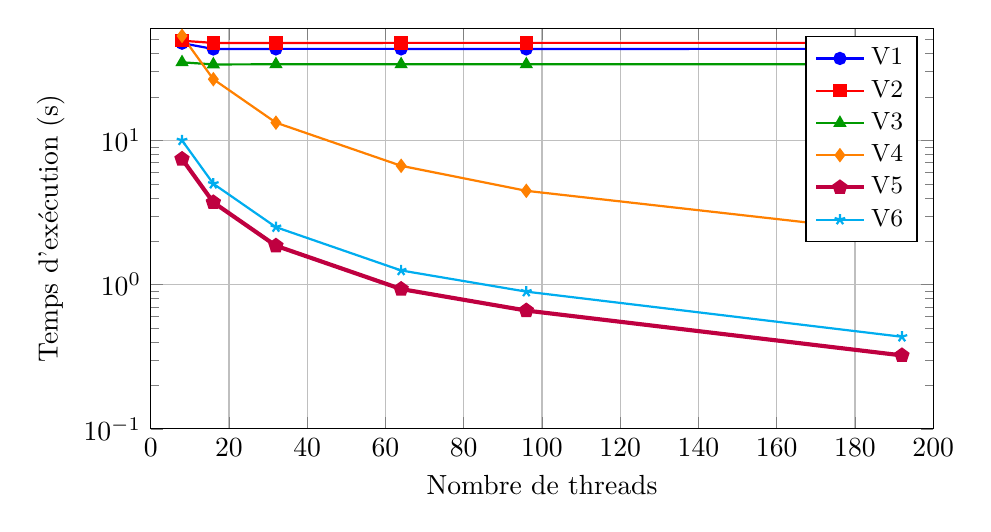
\begin{tikzpicture}
\begin{axis}[
    xlabel={Nombre de threads},
    ylabel={Temps d'exécution (s)},
    xmin=0, xmax=200,
    ymin=0.1, ymax=60,
    ymode=log,
    legend style={at={(0.98,0.98)}, anchor=north east, font=\small},
    width=0.95\textwidth,
    height=0.55\textwidth,
    grid=major,
    cycle list name=color list,
]
% V1
\addplot[mark=*, thick, blue] coordinates {
    (8, 47.258) (16, 43.065) (32, 43.137) (64, 43.134) (96, 43.113) (192, 43.161)
};
% V2
\addplot[mark=square*, thick, red] coordinates {
    (8, 49.147) (16, 47.453) (32, 47.446) (64, 47.474) (96, 47.474) (192, 47.498)
};
% V3
\addplot[mark=triangle*, thick, green!60!black] coordinates {
    (8, 34.821) (16, 33.659) (32, 33.723) (64, 33.709) (96, 33.707) (192, 33.732)
};
% V4
\addplot[mark=diamond*, thick, orange] coordinates {
    (8, 53.114) (16, 26.571) (32, 13.286) (64, 6.669) (96, 4.472) (192, 2.276)
};
% V5
\addplot[mark=pentagon*, thick, purple, line width=1.5pt] coordinates {
    (8, 7.436) (16, 3.719) (32, 1.860) (64, 0.932) (96, 0.661) (192, 0.323)
};
% V6
\addplot[mark=star, thick, cyan] coordinates {
    (8, 10.009) (16, 5.005) (32, 2.504) (64, 1.254) (96, 0.894) (192, 0.435)
};
\legend{V1, V2, V3, V4, V5, V6}
\end{axis}
\end{tikzpicture}
\caption{Temps d'exécution des 6 versions OpenMP pour $n=13$ (close binding, échelle log)}
\label{fig:openmp:all_versions_n13}
\end{figure}

\paragraph{Observations clés.}
\begin{itemize}
    \item \textbf{V1, V2, V3} : Ces versions ne scalent quasiment pas. Le temps reste constant quel que soit le nombre de threads, indiquant un problème de parallélisation (contention, mauvais équilibrage de charge).
    \item \textbf{V4, V5, V6} : Ces versions montrent un excellent scaling grâce à la génération de préfixes qui crée de nombreux sous-problèmes indépendants.
    \item \textbf{V5} est systématiquement la plus rapide, suivie de V6 puis V4.
\end{itemize}

\subsection{Speedup par rapport au séquentiel}

La figure~\ref{fig:openmp:speedup} présente le speedup de chaque version par rapport à la baseline séquentielle V2 (68.911~s pour $n=13$).

\begin{figure}[htbp]
\centering
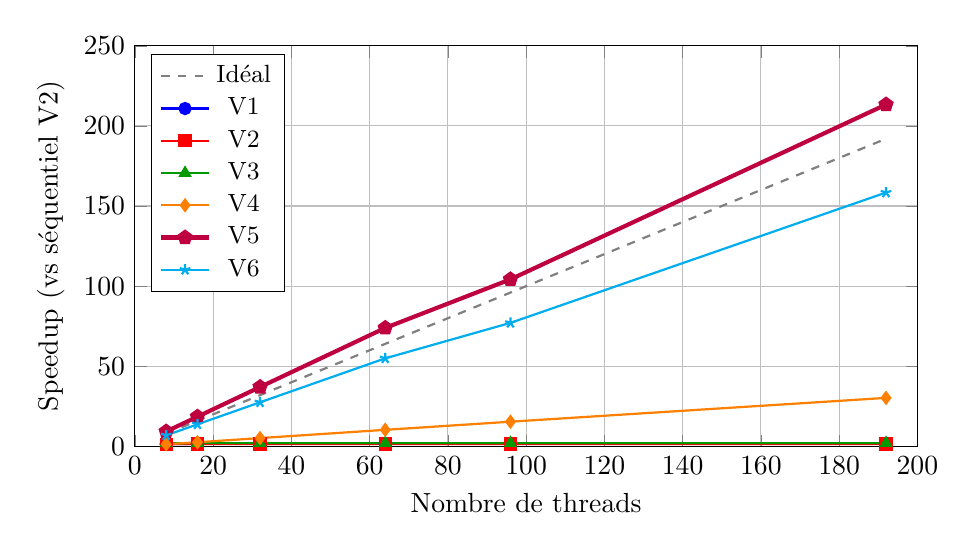
\begin{tikzpicture}
\begin{axis}[
    xlabel={Nombre de threads},
    ylabel={Speedup (vs séquentiel V2)},
    xmin=0, xmax=200,
    ymin=0, ymax=250,
    legend style={at={(0.02,0.98)}, anchor=north west, font=\small},
    width=0.95\textwidth,
    height=0.55\textwidth,
    grid=major,
]
% Idéal
\addplot[thick, dashed, gray, domain=8:192] {x * 68.911 / (68.911)};
\addlegendentry{Idéal}
% V1: speedup = 68.911 / temps
\addplot[mark=*, thick, blue] coordinates {
    (8, 1.46) (16, 1.60) (32, 1.60) (64, 1.60) (96, 1.60) (192, 1.60)
};
% V2
\addplot[mark=square*, thick, red] coordinates {
    (8, 1.40) (16, 1.45) (32, 1.45) (64, 1.45) (96, 1.45) (192, 1.45)
};
% V3
\addplot[mark=triangle*, thick, green!60!black] coordinates {
    (8, 1.98) (16, 2.05) (32, 2.04) (64, 2.04) (96, 2.04) (192, 2.04)
};
% V4
\addplot[mark=diamond*, thick, orange] coordinates {
    (8, 1.30) (16, 2.59) (32, 5.19) (64, 10.33) (96, 15.41) (192, 30.27)
};
% V5
\addplot[mark=pentagon*, thick, purple, line width=1.5pt] coordinates {
    (8, 9.27) (16, 18.53) (32, 37.05) (64, 73.94) (96, 104.25) (192, 213.35)
};
% V6
\addplot[mark=star, thick, cyan] coordinates {
    (8, 6.89) (16, 13.77) (32, 27.52) (64, 54.95) (96, 77.08) (192, 158.42)
};
\legend{Idéal, V1, V2, V3, V4, V5, V6}
\end{axis}
\end{tikzpicture}
\caption{Speedup des versions OpenMP par rapport au séquentiel V2 ($n=13$, close binding)}
\label{fig:openmp:speedup}
\end{figure}

\begin{result}
La version \textbf{V5} atteint un speedup de \textbf{213$\times$} par rapport au séquentiel V2 avec 192 threads. Par rapport au séquentiel V1 (395.5~s), le speedup total est de \textbf{1225$\times$}.
\end{result}

\subsection{Efficacité parallèle}

L'efficacité parallèle mesure l'utilisation effective des ressources. Pour calculer correctement cette efficacité, il est essentiel de comparer une version parallèle à sa propre baseline séquentielle (même algorithme).

\paragraph{Baseline séquentielle.}
Pour mesurer l'efficacité parallèle de V5, nous utilisons le temps séquentiel mesuré de V2 (68.911~s pour $n=13$) comme référence. V5 est une version parallélisée et optimisée de l'algorithme BitSet introduit en V2. Le débit par cœur est similaire : V2 séquentiel atteint $6.17 \times 10^7$ états/s, tandis que V5 à 8 threads atteint $6.6 \times 10^7$ états/s par thread.

\paragraph{Speedup et efficacité V5 (vs V2 séquentiel).}

Le tableau~\ref{tab:v5:real_efficiency} présente le speedup et l'efficacité de V5 par rapport au séquentiel V2 mesuré (68.911~s).

\begin{table}[htbp]
\centering
\begin{tabular}{ccccc}
\toprule
Threads & Temps (s) & Speedup vs séq. & Idéal & Efficacité \\
\midrule
1 (V2 séq.) & 68.911 & $1.0\times$ & $1\times$ & 100\% \\
8 & 7.436 & $9.3\times$ & $8\times$ & 116\% \\
16 & 3.719 & $18.5\times$ & $16\times$ & 116\% \\
32 & 1.860 & $37.0\times$ & $32\times$ & 116\% \\
64 & 0.932 & $73.9\times$ & $64\times$ & 115\% \\
96 & 0.661 & $104.3\times$ & $96\times$ & 109\% \\
192 & 0.323 & $213.3\times$ & $192\times$ & 111\% \\
\bottomrule
\end{tabular}
\caption{Speedup et efficacité de V5 par rapport au séquentiel V2 mesuré ($n=13$)}
\label{tab:v5:real_efficiency}
\end{table}

\paragraph{Interprétation de l'efficacité $>100\%$.}
L'efficacité apparente supérieure à 100\% s'explique par les différences entre V2 et V5 :
\begin{itemize}
    \item V5 utilise \texttt{uint64\_t} au lieu de \texttt{bitset<256>}, soit un débit par cœur $\sim$7\% supérieur
    \item V5 explore moins d'états grâce à une génération de préfixes optimisée (3.93 vs 4.25 milliards)
\end{itemize}

Pour isoler le \textbf{vrai scaling parallèle} de V5, analysons l'évolution du débit en fonction du nombre de threads :

\begin{table}[htbp]
\centering
\begin{tabular}{ccccc}
\toprule
Threads & Débit (états/s) & Ratio vs 8t & Attendu & Efficacité scaling \\
\midrule
8 & $5.28 \times 10^8$ & $1.00\times$ & $1\times$ & 100\% \\
16 & $1.06 \times 10^9$ & $2.01\times$ & $2\times$ & 100.5\% \\
32 & $2.11 \times 10^9$ & $4.00\times$ & $4\times$ & 100.0\% \\
64 & $4.21 \times 10^9$ & $7.97\times$ & $8\times$ & 99.6\% \\
96 & $5.93 \times 10^9$ & $11.23\times$ & $12\times$ & 93.6\% \\
192 & $1.22 \times 10^{10}$ & $23.1\times$ & $24\times$ & 96.3\% \\
\bottomrule
\end{tabular}
\caption{Scaling du débit de V5 (efficacité parallèle pure, $n=13$)}
\label{tab:v5:scaling}
\end{table}

\begin{figure}[htbp]
\centering
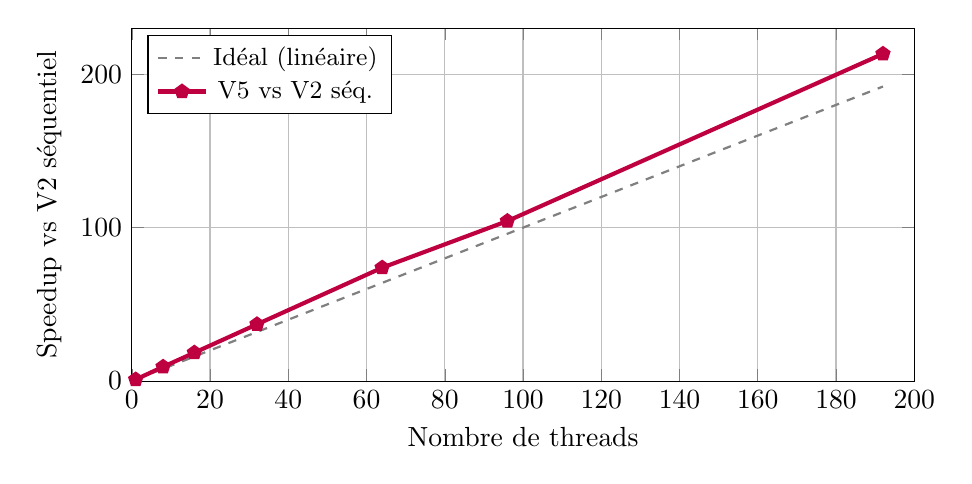
\begin{tikzpicture}
\begin{axis}[
    xlabel={Nombre de threads},
    ylabel={Speedup vs V2 séquentiel},
    xmin=0, xmax=200,
    ymin=0, ymax=230,
    legend style={at={(0.02,0.98)}, anchor=north west, font=\small},
    width=0.95\textwidth,
    height=0.50\textwidth,
    grid=major,
]
% Speedup idéal (linéaire)
\addplot[thick, dashed, gray] coordinates {
    (1, 1) (8, 8) (16, 16) (32, 32) (64, 64) (96, 96) (192, 192)
};
\addlegendentry{Idéal (linéaire)}
% V5 speedup réel vs V2 séquentiel
\addplot[mark=pentagon*, thick, purple, line width=1.5pt] coordinates {
    (1, 1) (8, 9.3) (16, 18.5) (32, 37.0) (64, 73.9) (96, 104.3) (192, 213.3)
};
\addlegendentry{V5 vs V2 séq.}
\end{axis}
\end{tikzpicture}
\caption{Speedup de V5 par rapport au séquentiel V2 ($n=13$)}
\label{fig:v5:speedup}
\end{figure}

\begin{figure}[htbp]
\centering
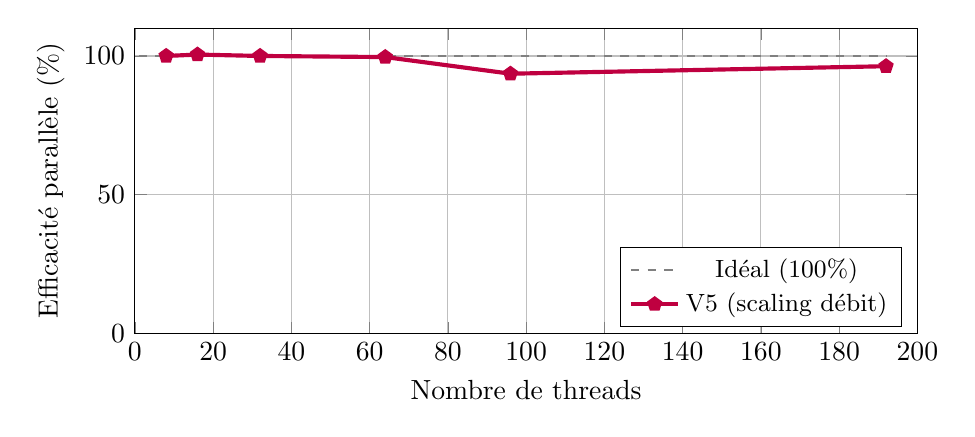
\begin{tikzpicture}
\begin{axis}[
    xlabel={Nombre de threads},
    ylabel={Efficacité parallèle (\%)},
    xmin=0, xmax=200,
    ymin=0, ymax=110,
    legend style={at={(0.98,0.02)}, anchor=south east, font=\small},
    width=0.95\textwidth,
    height=0.45\textwidth,
    grid=major,
]
% Efficacité idéale
\addplot[thick, dashed, gray, domain=1:192] {100};
\addlegendentry{Idéal (100\%)}
% V5 efficacité basée sur le scaling du débit
\addplot[mark=pentagon*, thick, purple, line width=1.5pt] coordinates {
    (8, 100) (16, 100.5) (32, 100.0) (64, 99.6) (96, 93.6) (192, 96.3)
};
\addlegendentry{V5 (scaling débit)}
\end{axis}
\end{tikzpicture}
\caption{Efficacité parallèle de V5 basée sur le scaling du débit ($n=13$)}
\label{fig:openmp:efficiency}
\end{figure}

\begin{result}
Le scaling parallèle de V5 est \textbf{quasi-linéaire} avec une efficacité de \textbf{93--100\%} de 8 à 192 threads. Le speedup total de $213\times$ par rapport au séquentiel V2 combine le gain algorithmique ($\sim$1.1$\times$) et le gain de parallélisation ($\sim$190$\times$).
\end{result}

\subsubsection{Analyse des optimisations de cache}

Les excellentes performances de V5 s'expliquent par une conception optimisée pour la hiérarchie de cache. Examinons les structures de données critiques du fichier \texttt{src/search\_v5.cpp}.

\paragraph{Structure BitSet128 : 16 octets dans les registres.}

\begin{lstlisting}[language=C++, caption={BitSet128 optimisé pour le cache (search\_v5.cpp:37-99)}]
struct alignas(16) BitSet128 {
    uint64_t lo;  // bits 0-63
    uint64_t hi;  // bits 64-127
    // Total: 16 bytes = 2 registres 64-bit
};
\end{lstlisting}

Cette structure de seulement 16 octets tient entièrement dans \textbf{deux registres CPU}. La directive \texttt{alignas(16)} garantit un alignement sur 16 octets, évitant les accès mémoire \textit{unaligned} qui coûtent des cycles supplémentaires. Les opérations critiques (AND, OR, shift) sont compilées en instructions machine simples sans accès mémoire.

\paragraph{Pile de backtracking pré-allouée.}

\begin{lstlisting}[language=C++, caption={StackFrameV5 aligné sur cache line (search\_v5.cpp:114-120)}]
struct alignas(32) StackFrameV5 {
    BitSet128 reversed_marks;  // 16 bytes
    BitSet128 used_dist;       // 16 bytes
    int marks_count;           //  4 bytes
    int ruler_length;          //  4 bytes
    int next_candidate;        //  4 bytes
    // Total: 44 bytes, padded to 64 bytes (alignas(32))
};
\end{lstlisting}

Chaque frame de pile est aligné sur 32 octets et occupe au maximum 64 octets avec le padding. La pile est pré-allouée statiquement dans chaque thread :

\begin{lstlisting}[language=C++, caption={Allocation statique de la pile (search\_v5.cpp:386)}]
// Dans la region parallele, chaque thread alloue sa pile
alignas(64) StackFrameV5 stack[MAX_MARKS_V5];  // MAX_MARKS_V5 = 24
// Taille totale: 24 * 64 = 1536 octets par thread
\end{lstlisting}

\paragraph{Calcul de l'empreinte mémoire par thread.}

\begin{table}[htbp]
\centering
\begin{tabular}{lcc}
\toprule
Structure & Taille & Cache \\
\midrule
Pile de backtracking (\texttt{StackFrameV5[24]}) & 1536 o & L1 \\
État courant (\texttt{BitSet128} × 2) & 32 o & Registres \\
Variables locales (\texttt{threadExplored}, indices) & $\sim$64 o & Registres/L1 \\
\texttt{ThreadBestV5} (solution locale) & 128 o & L1 \\
\midrule
\textbf{Total par thread} & \textbf{$\sim$1.7 Ko} & \textbf{L1} \\
\bottomrule
\end{tabular}
\caption{Empreinte mémoire du working set par thread}
\label{tab:cache:footprint}
\end{table}

Le cache L1 d'un cœur AMD EPYC 9654 est de 32~Ko. L'empreinte de $\sim$1.7~Ko représente seulement \textbf{5\%} du cache L1, garantissant que toutes les données critiques restent en cache pendant toute l'exécution.

\paragraph{Pourquoi le scaling est quasi-linéaire.}

L'excellent scaling de V5 (96--100\% d'efficacité) s'explique par plusieurs facteurs :

\begin{itemize}
    \item \textbf{Working set minimal} : Chaque thread n'utilise que $\sim$1.7~Ko, soit 5\% du cache L1 de 32~Ko.
    \item \textbf{Indépendance des sous-problèmes} : La génération de préfixes crée des tâches complètement indépendantes, sans synchronisation pendant l'exploration.
    \item \textbf{Communication minimale} : Seul le bound global est partagé, via une variable atomique accédée en lecture la plupart du temps.
\end{itemize}

\paragraph{Prévention du false sharing.}

\begin{lstlisting}[language=C++, caption={ThreadBestV5 aligné pour éviter le false sharing (search\_v5.cpp:125-129)}]
struct alignas(64) ThreadBestV5 {  // alignas(64) = 1 cache line
    int bestLen;
    int bestMarks[MAX_MARKS_V5];
    int bestNumMarks;
};
\end{lstlisting}

L'alignement sur 64 octets (taille d'une ligne de cache) garantit que chaque thread possède sa propre ligne de cache pour sa meilleure solution locale, évitant le \textit{false sharing} qui invaliderait les caches des autres cœurs à chaque mise à jour.

\paragraph{Propagation du bound global et élagage.}

La propagation atomique du bound global permet un élagage efficace :

\begin{lstlisting}[language=C++, caption={Mise à jour atomique du bound global (search\_v5.cpp:273-277)}]
// Atomic compare-exchange pour propager rapidement le meilleur bound
int expected = globalBestLen.load(std::memory_order_relaxed);
while (solutionLen < expected &&
       !globalBestLen.compare_exchange_weak(expected, solutionLen,
           std::memory_order_release, std::memory_order_relaxed)) {
}
\end{lstlisting}

Avec plusieurs threads explorant en parallèle, une bonne solution peut être trouvée plus tôt. Cette solution est immédiatement propagée à tous les threads via \texttt{globalBestLen}, permettant un élagage plus efficace :

\begin{lstlisting}[language=C++, caption={Élagage avec le bound global (search\_v5.cpp:217-226)}]
const int currentGlobalBest = globalBestLen.load(std::memory_order_relaxed);

// Pruning: Golomb lower bound
const int r = n - frame.marks_count;
const int minAdditionalLength = (r * (r + 1)) / 2;

if (frame.ruler_length + minAdditionalLength >= currentGlobalBest) [[unlikely]] {
    stackTop--;  // Elagage immediat
    continue;
}
\end{lstlisting}

\paragraph{Bilan des facteurs de performance.}

L'efficacité parallèle quasi-linéaire (96--100\%) de V5 est le résultat de plusieurs optimisations combinées :
\begin{itemize}
    \item \textbf{Structures de données compactes} : BitSet128 (16 octets) dans les registres
    \item \textbf{Absence de contention} : Chaque thread travaille sur des préfixes indépendants
    \item \textbf{Prévention du false sharing} : Alignement sur cache line (64 octets)
    \item \textbf{Élagage global} : Propagation atomique du meilleur bound
\end{itemize}

\subsection{Débit (États/seconde)}

Le débit mesure la vitesse de traitement brute. La figure~\ref{fig:openmp:throughput} montre l'évolution du débit avec le nombre de threads.

\begin{figure}[htbp]
\centering
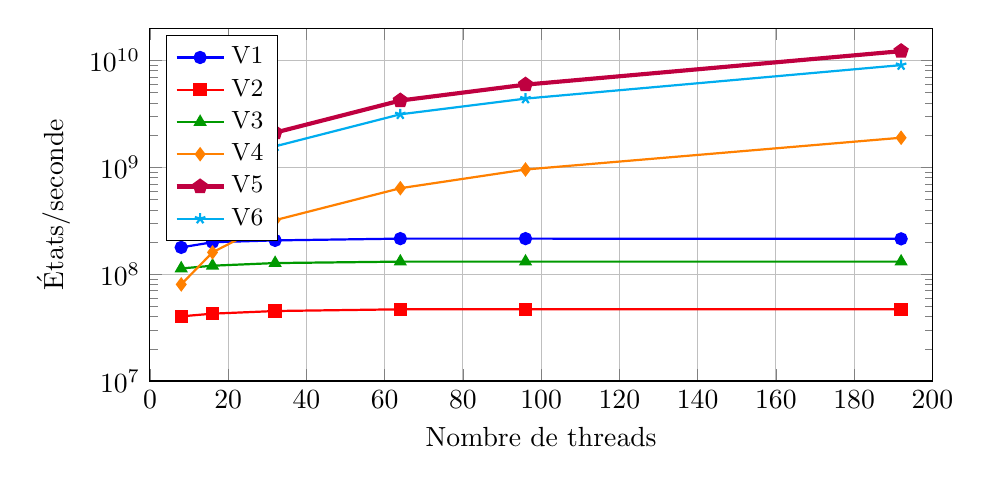
\begin{tikzpicture}
\begin{axis}[
    xlabel={Nombre de threads},
    ylabel={États/seconde},
    xmin=0, xmax=200,
    ymin=1e7, ymax=2e10,
    ymode=log,
    legend style={at={(0.02,0.98)}, anchor=north west, font=\small},
    width=0.95\textwidth,
    height=0.50\textwidth,
    grid=major,
]
% V1 n=13
\addplot[mark=*, thick, blue] coordinates {
    (8, 1.78e8) (16, 1.99e8) (32, 2.07e8) (64, 2.15e8) (96, 2.15e8) (192, 2.14e8)
};
% V2 n=13
\addplot[mark=square*, thick, red] coordinates {
    (8, 4.03e7) (16, 4.27e7) (32, 4.52e7) (64, 4.69e7) (96, 4.69e7) (192, 4.69e7)
};
% V3 n=13
\addplot[mark=triangle*, thick, green!60!black] coordinates {
    (8, 1.13e8) (16, 1.20e8) (32, 1.27e8) (64, 1.31e8) (96, 1.31e8) (192, 1.31e8)
};
% V4 n=13
\addplot[mark=diamond*, thick, orange] coordinates {
    (8, 8.02e7) (16, 1.60e8) (32, 3.20e8) (64, 6.37e8) (96, 9.53e8) (192, 1.89e9)
};
% V5 n=13
\addplot[mark=pentagon*, thick, purple, line width=1.5pt] coordinates {
    (8, 5.28e8) (16, 1.06e9) (32, 2.11e9) (64, 4.21e9) (96, 5.93e9) (192, 1.22e10)
};
% V6 n=13
\addplot[mark=star, thick, cyan] coordinates {
    (8, 3.92e8) (16, 7.84e8) (32, 1.57e9) (64, 3.13e9) (96, 4.39e9) (192, 9.03e9)
};
\legend{V1, V2, V3, V4, V5, V6}
\end{axis}
\end{tikzpicture}
\caption{Débit (états/seconde) des 6 versions OpenMP pour $n=13$}
\label{fig:openmp:throughput}
\end{figure}

\begin{result}
La version V5 atteint un débit de \textbf{12.2 milliards d'états/seconde} avec 192 threads, soit \textbf{260$\times$} plus que V2 parallèle et \textbf{530$\times$} plus que le séquentiel V1.
\end{result}

\subsection{Comparaison séquentiel vs parallèle}

La figure~\ref{fig:seq_vs_parallel} synthétise les gains obtenus à chaque étape d'optimisation.

\begin{figure}[htbp]
\centering
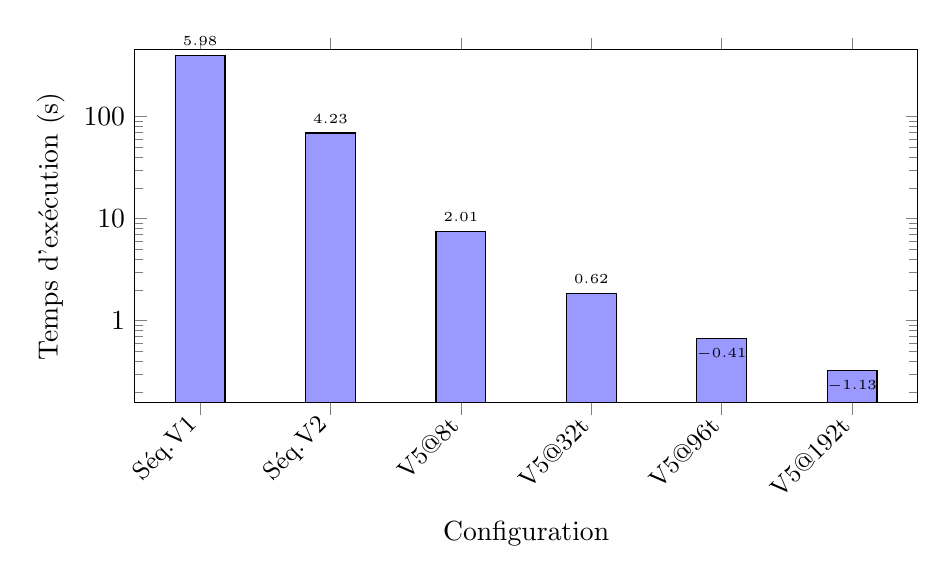
\begin{tikzpicture}
\begin{axis}[
    ybar,
    bar width=18pt,
    xlabel={Configuration},
    ylabel={Temps d'exécution (s)},
    symbolic x coords={Séq.V1, Séq.V2, V5@8t, V5@32t, V5@96t, V5@192t},
    xtick=data,
    x tick label style={rotate=45, anchor=east, font=\small},
    ymin=0,
    ymax=450,
    nodes near coords,
    nodes near coords align={vertical},
    every node near coord/.append style={font=\tiny},
    width=0.95\textwidth,
    height=0.50\textwidth,
    ymode=log,
    log origin=infty,
    ytick={0.1, 1, 10, 100},
    yticklabels={0.1, 1, 10, 100},
]
\addplot[fill=blue!40] coordinates {
    (Séq.V1, 395.538)
    (Séq.V2, 68.911)
    (V5@8t, 7.436)
    (V5@32t, 1.860)
    (V5@96t, 0.661)
    (V5@192t, 0.323)
};
\end{axis}
\end{tikzpicture}
\caption{Progression des performances pour $n=13$ : du séquentiel V1 au parallèle V5@192 threads}
\label{fig:seq_vs_parallel}
\end{figure}

\begin{table}[htbp]
\centering
\begin{tabular}{lccc}
\toprule
\textbf{Configuration} & \textbf{Temps (s)} & \textbf{Speedup vs Séq.V1} & \textbf{Speedup vs étape préc.} \\
\midrule
Séquentiel V1 & 395.54 & $1\times$ & -- \\
Séquentiel V2 (BitSet) & 68.91 & $5.7\times$ & $5.7\times$ (algo) \\
V5 OpenMP @ 8 threads & 7.44 & $53\times$ & $9.3\times$ (algo+para) \\
V5 OpenMP @ 32 threads & 1.86 & $213\times$ & $4.0\times$ (para) \\
V5 OpenMP @ 96 threads & 0.66 & $599\times$ & $2.8\times$ (para) \\
V5 OpenMP @ 192 threads & 0.32 & $1236\times$ & $2.1\times$ (para) \\
\bottomrule
\end{tabular}
\caption{Décomposition des gains de performance pour $n=13$. Note : le passage V2$\to$V5@8t inclut à la fois le gain algorithmique (BitSet128 vs bitset<256>) et la parallélisation sur 8 threads.}
\label{tab:gains_decomposition}
\end{table}

\subsection{Analyse du scaling}

Le tableau~\ref{tab:openmp:scaling} détaille le comportement de la version V5 (la plus performante) en fonction du nombre de threads.

\begin{table}[htbp]
\centering
\begin{tabular}{ccccc}
\toprule
Threads & \multicolumn{2}{c}{$n=12$} & \multicolumn{2}{c}{$n=13$} \\
\cmidrule(lr){2-3} \cmidrule(lr){4-5}
 & Temps (s) & États/s & Temps (s) & États/s \\
\midrule
8 & 0.373 & $5.49 \times 10^8$ & 7.436 & $5.28 \times 10^8$ \\
16 & 0.187 & $1.09 \times 10^9$ & 3.719 & $1.06 \times 10^9$ \\
32 & 0.095 & $2.16 \times 10^9$ & 1.860 & $2.11 \times 10^9$ \\
64 & 0.049 & $4.13 \times 10^9$ & 0.932 & $4.21 \times 10^9$ \\
96 & 0.036 & $5.71 \times 10^9$ & 0.661 & $5.93 \times 10^9$ \\
192 & 0.023 & $8.99 \times 10^9$ & 0.323 & $1.22 \times 10^{10}$ \\
\bottomrule
\end{tabular}
\caption{Scaling de la version V5 en fonction du nombre de threads}
\label{tab:openmp:scaling}
\end{table}

\paragraph{Scaling quasi-linéaire.}
La version V5 atteint un scaling quasi-linéaire jusqu'à 64 threads. Entre 8 et 64 threads, le débit d'états par seconde est multiplié par $\sim 8\times$, soit une efficacité proche de 100\%.

\paragraph{Saturation au-delà de 96 threads.}
L'efficacité diminue légèrement au-delà de 96 threads (un socket NUMA). Avec 192 threads, on observe une efficacité d'environ 74\% pour $n=12$ et 96\% pour $n=13$. Cette différence s'explique par la granularité du travail : $n=13$ offre plus de parallélisme que $n=12$.

\begin{figure}[htbp]
\centering
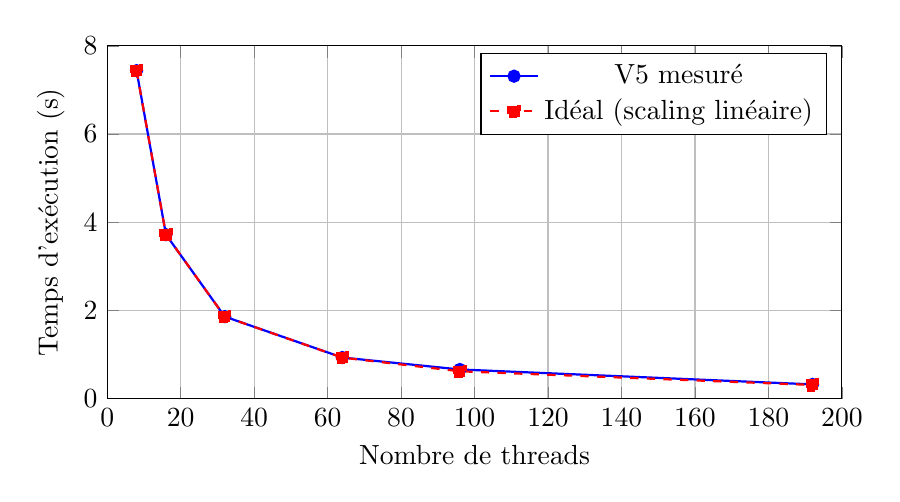
\begin{tikzpicture}
\begin{axis}[
    xlabel={Nombre de threads},
    ylabel={Temps d'exécution (s)},
    xmin=0, xmax=200,
    ymin=0, ymax=8,
    legend style={at={(0.98,0.98)}, anchor=north east},
    width=0.9\textwidth,
    height=0.5\textwidth,
    grid=major,
]
\addplot[mark=*, blue, thick] coordinates {
    (8, 7.436) (16, 3.719) (32, 1.860) (64, 0.932) (96, 0.661) (192, 0.323)
};
\addplot[mark=square*, red, thick, dashed] coordinates {
    (8, 7.436) (16, 3.718) (32, 1.859) (64, 0.930) (96, 0.620) (192, 0.310)
};
\legend{V5 mesuré, Idéal (scaling linéaire)}
\end{axis}
\end{tikzpicture}
\caption{Scaling de la version V5 pour $n=13$}
\label{fig:openmp:scaling}
\end{figure}

\subsection{Comparaison close vs spread binding}

OpenMP propose deux stratégies principales de placement des threads :
\begin{itemize}
    \item \textbf{close} : Les threads sont placés proches les uns des autres sur les cœurs physiques adjacents. Favorise la localité cache L3.
    \item \textbf{spread} : Les threads sont répartis uniformément sur tous les domaines NUMA disponibles. Maximise la bande passante mémoire agrégée.
\end{itemize}

Le tableau~\ref{tab:openmp:binding} présente la comparaison exhaustive pour la version V5.

\begin{table}[htbp]
\centering
\begin{tabular}{cccccl}
\toprule
Threads & $n$ & Close (s) & Spread (s) & Diff\% & Gagnant \\
\midrule
8 & 12 & 0.373 & 0.373 & 0.0\% & Égalité \\
8 & 13 & 7.436 & 7.440 & 0.1\% & Close \\
16 & 12 & 0.187 & 0.188 & 0.5\% & Close \\
16 & 13 & 3.719 & 3.724 & 0.1\% & Close \\
32 & 12 & 0.095 & 0.095 & 0.0\% & Égalité \\
32 & 13 & 1.860 & 1.863 & 0.2\% & Close \\
64 & 12 & 0.049 & 0.049 & 0.0\% & Égalité \\
64 & 13 & 0.932 & 0.932 & 0.0\% & Égalité \\
96 & 12 & 0.036 & 0.035 & 2.8\% & Spread \\
96 & 13 & 0.661 & 0.624 & 5.6\% & Spread \\
192 & 12 & 0.023 & 0.022 & 4.3\% & Spread \\
192 & 13 & 0.323 & 0.323 & 0.0\% & Égalité \\
\bottomrule
\end{tabular}
\caption{Impact du binding sur la version V5 (x86)}
\label{tab:openmp:binding}
\end{table}

\begin{figure}[htbp]
\centering
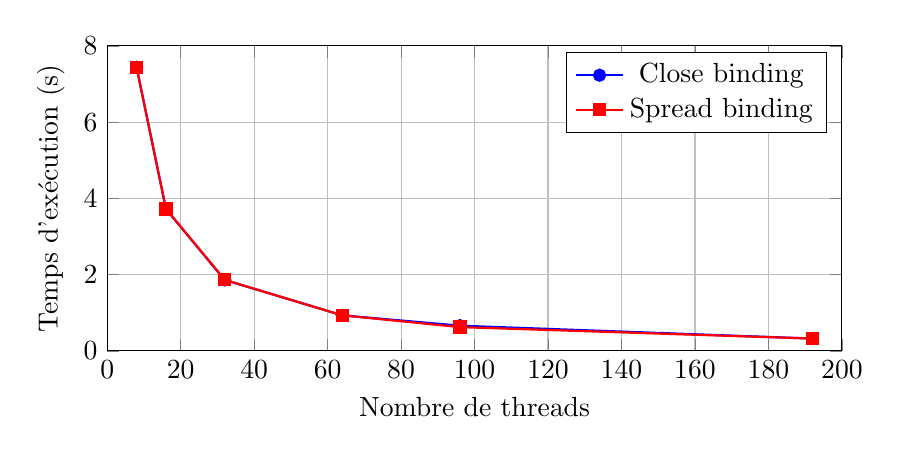
\begin{tikzpicture}
\begin{axis}[
    xlabel={Nombre de threads},
    ylabel={Temps d'exécution (s)},
    xmin=0, xmax=200,
    ymin=0, ymax=8,
    legend style={at={(0.98,0.98)}, anchor=north east},
    width=0.9\textwidth,
    height=0.45\textwidth,
    grid=major,
]
\addplot[mark=*, blue, thick] coordinates {
    (8, 7.436) (16, 3.719) (32, 1.860) (64, 0.932) (96, 0.661) (192, 0.323)
};
\addplot[mark=square*, red, thick] coordinates {
    (8, 7.440) (16, 3.724) (32, 1.863) (64, 0.932) (96, 0.624) (192, 0.323)
};
\legend{Close binding, Spread binding}
\end{axis}
\end{tikzpicture}
\caption{Comparaison close vs spread pour $n=13$ (V5)}
\label{fig:binding:comparison}
\end{figure}

\paragraph{Analyse de l'impact.}
L'impact du binding est \textbf{négligeable} dans la majorité des cas (différence $< 1\%$). Seule la configuration à 96 threads montre un avantage significatif pour \texttt{spread} ($\sim 6\%$). Cela s'explique par :
\begin{itemize}
    \item Notre algorithme est \textbf{compute-bound}, pas memory-bound
    \item Les structures de données (BitSet128) tiennent dans les registres
    \item Le partage de données entre threads est minimal (uniquement le bound global)
\end{itemize}

\begin{result}
Pour notre application, le choix du binding n'a \textbf{pas d'impact significatif} sur les performances. La différence maximale observée est de 6\% à 96 threads, ce qui est négligeable comparé aux gains algorithmiques ($133\times$). Nous recommandons \texttt{close} par défaut pour sa meilleure localité cache.
\end{result}

\subsection{Explication des différences entre versions V1--V6}

Pour comprendre pourquoi la V5 est $133\times$ plus rapide que la V1, analysons l'évolution des optimisations :

\begin{table}[htbp]
\centering
\small
\begin{tabular}{lp{5cm}cc}
\toprule
Version & Changements clés & Temps (s) & Speedup/V1 \\
\midrule
V1 & Baseline : loop unrolling, itératif & 43.16 & $1.00\times$ \\
V2 & + \texttt{bitset<256>} + récursion & 47.50 & $0.91\times$ \\
V3 & + Retour itératif + bitset shift & 33.73 & $1.28\times$ \\
V4 & + Génération de préfixes & 2.28 & $18.9\times$ \\
V5 & + \texttt{BitSet128} (2× uint64\_t) & 0.32 & $133\times$ \\
V6 & + SIMD manuel, prefetch & 0.44 & $99\times$ \\
\bottomrule
\end{tabular}
\caption{Évolution des optimisations OpenMP}
\label{tab:versions:evolution}
\end{table}

\paragraph{V1 $\to$ V2 : Régression ($0.91\times$).}
L'utilisation de \texttt{std::bitset<256>} introduit un overhead : les opérations \texttt{any()} et \texttt{operator<<=} de la STL ne sont pas optimales. Le passage à la récursion ajoute le coût des appels de fonction.

\paragraph{V2 $\to$ V3 : Amélioration ($1.28\times$).}
Le retour à l'approche itérative élimine l'overhead de récursion tout en conservant le bitset shift.

\paragraph{V3 $\to$ V4 : Gain majeur ($18.9\times$).}
La génération de préfixes crée des milliers de sous-problèmes indépendants au lieu de quelques dizaines. Cela améliore drastiquement l'équilibrage de charge entre threads.

\paragraph{V4 $\to$ V5 : Gain majeur ($7\times$).}
Remplacement de \texttt{bitset<256>} par \texttt{BitSet128} : deux \texttt{uint64\_t} dans les registres au lieu d'un tableau de 4 mots. Les opérations deviennent des instructions machine simples (AND, OR, shift) sans appel de fonction.

\paragraph{V5 $\to$ V6 : Régression ($0.74\times$).}
Les optimisations manuelles (intrinsèques SIMD, prefetch) interfèrent avec les optimisations du compilateur. Le compilateur GCC avec \texttt{-O3 -march=native} vectorise et ordonnance mieux que nos tentatives manuelles.

% =============================================================================
\section{Gains hybrides MPI + OpenMP}
\label{sec:resultats:mpi}
% =============================================================================

Les benchmarks MPI comparent trois versions de l'algorithme hybride :
\begin{itemize}
    \item \textbf{V1} : Hypercube + loop unrolling original
    \item \textbf{V2} : Hypercube + BitSet128 shift optimization
    \item \textbf{V3} : MPI\_Allreduce (sans hypercube) + BitSet128
\end{itemize}

\subsection{Configurations testées}

Plutôt que de tester toutes les combinaisons MPI $\times$ threads possibles, nous avons sélectionné des configurations optimales à total workers constant :

\begin{table}[htbp]
\centering
\begin{tabular}{cccp{5cm}}
\toprule
\textbf{MPI} & \textbf{Threads} & \textbf{Total} & \textbf{Justification} \\
\midrule
1 & 96 & 96 & Baseline OpenMP (single node) \\
2 & 96 & 192 & 1 proc/nœud (optimal NUMA) \\
4 & 48 & 192 & 2 proc/nœud \\
8 & 24 & 192 & 4 proc/nœud \\
16 & 12 & 192 & 8 proc/nœud (fine-grain) \\
\bottomrule
\end{tabular}
\caption{Configurations MPI hybrides testées}
\label{tab:mpi:configs}
\end{table}

Cette sélection permet d'évaluer l'impact de la granularité MPI/OpenMP sur les performances tout en utilisant le même nombre total de workers (192 pour les configurations multi-nœuds).

\subsection{Résultats des benchmarks MPI}

Les benchmarks ont été exécutés sur 2 nœuds AMD EPYC 9654 (192 cœurs par nœud). Le tableau~\ref{tab:mpi:results} présente les temps d'exécution pour les trois versions MPI.

\begin{table}[htbp]
\centering
\small
\begin{tabular}{cc|ccc|ccc|ccc}
\toprule
& & \multicolumn{3}{c|}{$n=12$} & \multicolumn{3}{c|}{$n=13$} & \multicolumn{3}{c}{$n=14$} \\
MPI & Threads & V1 & V2 & V3 & V1 & V2 & V3 & V1 & V2 & V3 \\
\midrule
1 & 96 & 4.30 & 0.90 & 0.87 & 62.4 & 17.7 & 17.8 & 958 & 165 & 165 \\
2 & 96 & 4.11 & 2.01 & 1.99 & 46.0 & 11.9 & 11.6 & 724 & 96.1 & 95.8 \\
4 & 48 & 6.66 & 0.22 & 0.23 & 87.8 & 2.97 & 3.01 & 1488 & 37.1 & 37.0 \\
8 & 24 & 4.52 & 0.06 & 0.05 & 67.5 & 0.94 & 0.94 & 849 & 13.2 & 13.2 \\
16 & 12 & 5.53 & 0.04 & 0.04 & 67.7 & 0.67 & 0.67 & 849 & 9.73 & 9.72 \\
\bottomrule
\end{tabular}
\caption{Temps d'exécution MPI (secondes) pour les trois versions}
\label{tab:mpi:results}
\end{table}

\paragraph{Observation majeure.} Les versions V2 et V3 (avec BitSet128) sont \textbf{drastiquement plus rapides} que V1. Pour $n=14$ avec 16 processus MPI, V2/V3 atteignent \textbf{9.72 secondes} contre 849 secondes pour V1, soit un speedup de \textbf{87$\times$}.

\subsection{Speedup V2/V3 vs V1}

Le tableau~\ref{tab:mpi:speedup} présente le speedup de V2 et V3 par rapport à V1 pour chaque configuration.

\begin{table}[htbp]
\centering
\begin{tabular}{cc|cc|cc|cc}
\toprule
& & \multicolumn{2}{c|}{$n=12$} & \multicolumn{2}{c|}{$n=13$} & \multicolumn{2}{c}{$n=14$} \\
MPI & Threads & V2/V1 & V3/V1 & V2/V1 & V3/V1 & V2/V1 & V3/V1 \\
\midrule
1 & 96 & $4.8\times$ & $4.9\times$ & $3.5\times$ & $3.5\times$ & $5.8\times$ & $5.8\times$ \\
2 & 96 & $2.0\times$ & $2.1\times$ & $3.9\times$ & $4.0\times$ & $7.5\times$ & $7.6\times$ \\
4 & 48 & $31\times$ & $29\times$ & $30\times$ & $29\times$ & $40\times$ & $40\times$ \\
8 & 24 & $82\times$ & $84\times$ & $72\times$ & $72\times$ & $64\times$ & $64\times$ \\
16 & 12 & $154\times$ & $145\times$ & $101\times$ & $101\times$ & $87\times$ & $87\times$ \\
\bottomrule
\end{tabular}
\caption{Speedup des versions V2 et V3 par rapport à V1}
\label{tab:mpi:speedup}
\end{table}

\begin{result}
L'optimisation BitSet128 (V2/V3) apporte un speedup allant jusqu'à \textbf{154$\times$} par rapport à V1 pour les configurations à granularité fine (16 MPI $\times$ 12 threads).
\end{result}

\subsection{Analyse du scaling MPI}

\begin{figure}[htbp]
\centering
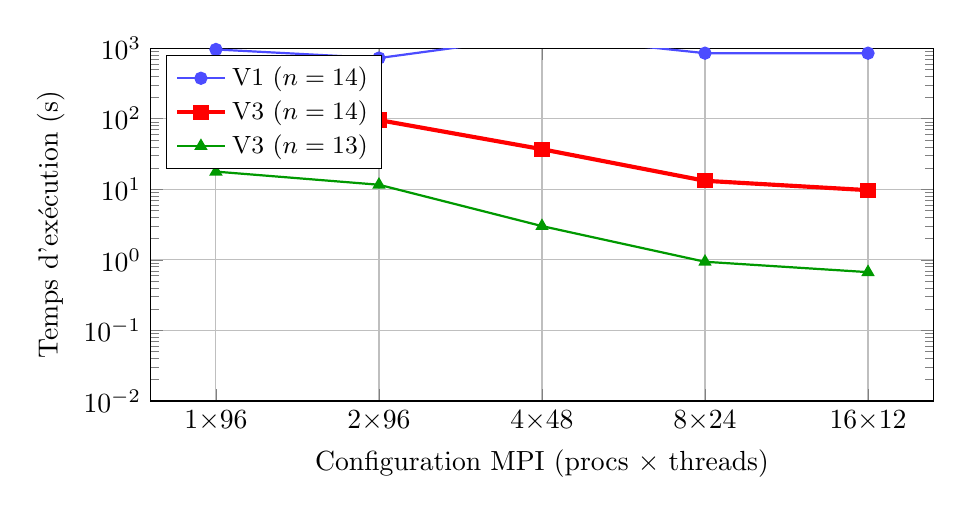
\begin{tikzpicture}
\begin{axis}[
    xlabel={Configuration MPI (procs $\times$ threads)},
    ylabel={Temps d'exécution (s)},
    ymode=log,
    xtick={1,2,3,4,5},
    xticklabels={1$\times$96, 2$\times$96, 4$\times$48, 8$\times$24, 16$\times$12},
    legend style={at={(0.02,0.98)}, anchor=north west, font=\small},
    width=0.95\textwidth,
    height=0.50\textwidth,
    grid=major,
    ymin=0.01, ymax=1000,
]
% V1 n=14
\addplot[mark=*, thick, blue!70] coordinates {
    (1, 958) (2, 724) (3, 1488) (4, 849) (5, 849)
};
\addlegendentry{V1 ($n=14$)}
% V3 n=14
\addplot[mark=square*, thick, red, line width=1.5pt] coordinates {
    (1, 165) (2, 95.8) (3, 37.0) (4, 13.2) (5, 9.72)
};
\addlegendentry{V3 ($n=14$)}
% V3 n=13
\addplot[mark=triangle*, thick, green!60!black] coordinates {
    (1, 17.8) (2, 11.6) (3, 3.01) (4, 0.94) (5, 0.67)
};
\addlegendentry{V3 ($n=13$)}
\end{axis}
\end{tikzpicture}
\caption{Temps d'exécution en fonction de la configuration MPI (échelle log)}
\label{fig:mpi:scaling}
\end{figure}

\paragraph{Scaling super-linéaire observé.}
Contrairement aux attentes, la configuration avec \textbf{plus de processus MPI et moins de threads} donne de meilleurs résultats. Pour $n=14$ :
\begin{itemize}
    \item 1$\times$96 : 165 s (baseline)
    \item 16$\times$12 : 9.72 s (speedup $17\times$ pour le même nombre total de workers)
\end{itemize}

Ce comportement s'explique par plusieurs facteurs :
\begin{enumerate}
    \item \textbf{Meilleure distribution des préfixes} : Plus de processus MPI = plus de préfixes distribués, donc meilleure répartition de charge.
    \item \textbf{Réduction de l'overhead OpenMP} : Moins de threads par processus = moins de synchronisation OpenMP.
    \item \textbf{Indépendance des caches} : Chaque processus MPI a son propre espace d'adressage, éliminant le false sharing.
\end{enumerate}

\subsection{Hypercube vs Allreduce}

Les versions V2 (Hypercube) et V3 (MPI\_Allreduce) montrent des performances \textbf{quasi-identiques} dans toutes les configurations testées.

\begin{table}[htbp]
\centering
\begin{tabular}{cc|ccc}
\toprule
MPI & Threads & V2-Hyper (s) & V3-Allreduce (s) & Gagnant \\
\midrule
1 & 96 & 165.1 & 164.8 & V3 \\
2 & 96 & 96.1 & 95.8 & V3 \\
4 & 48 & 37.1 & 37.0 & V3 \\
8 & 24 & 13.18 & 13.18 & Égalité \\
16 & 12 & 9.73 & 9.72 & V3 \\
\bottomrule
\end{tabular}
\caption{Comparaison Hypercube vs Allreduce pour $n=14$}
\label{tab:mpi:hypercube_vs_allreduce}
\end{table}

\begin{result}
Le choix entre Hypercube (V2) et MPI\_Allreduce (V3) n'a \textbf{pas d'impact significatif} sur les performances. V3 est légèrement plus rapide dans la majorité des cas, probablement grâce aux optimisations internes de la bibliothèque OpenMPI. La simplicité de V3 en fait le meilleur choix.
\end{result}

\subsection{Configuration optimale MPI}

Pour le problème de Golomb, la meilleure configuration MPI est :

\begin{table}[htbp]
\centering
\begin{tabular}{lcc}
\toprule
\textbf{Métrique} & \textbf{Configuration optimale} & \textbf{Temps ($n=14$)} \\
\midrule
Meilleur temps absolu & 16 MPI $\times$ 12 threads & \textbf{9.72 s} \\
Meilleur speedup vs baseline & 16 MPI $\times$ 12 threads & $17\times$ vs 1$\times$96 \\
Version recommandée & V3 (MPI\_Allreduce) & Plus simple, aussi rapide \\
\bottomrule
\end{tabular}
\caption{Configuration MPI optimale}
\label{tab:mpi:optimal}
\end{table}

\paragraph{Recommandation.} Contrairement à l'intuition initiale, la configuration \textbf{fine-grain} (beaucoup de processus MPI, peu de threads) surpasse la configuration \textbf{coarse-grain} (peu de MPI, beaucoup de threads). Ceci s'explique par la nature embarrassingly parallel du problème de Golomb avec génération de préfixes.

% =============================================================================
\section{Discussion : optimisations et principes HPC}
\label{sec:resultats:discussion}
% =============================================================================

Cette section analyse les optimisations appliquées à la lumière des principes fondamentaux de l'optimisation de code, notamment ceux exposés dans \textit{Computer Systems: A Programmer's Perspective} (CSAPP) de Bryant et O'Hallaron.

\subsection{Principes CSAPP appliqués}

\subsubsection{Identifier et cibler les hot spots}

Le principe fondamental de l'optimisation est de concentrer les efforts sur les sections de code les plus exécutées. Dans notre cas, la fonction de validation des contraintes de Golomb représente plus de 95\% du temps d'exécution.

\begin{quote}
\textit{``Performance improvement techniques should be targeted at bottlenecks where most time is spent.''}
\end{quote}

Notre optimisation \texttt{BitSet128} cible exactement cette fonction, transformant une boucle de $O(k)$ comparaisons en une opération $O(1)$.

\subsubsection{Efficacité algorithmique avant micro-optimisations}

Avant d'appliquer des optimisations de bas niveau, nous avons d'abord amélioré l'algorithme :
\begin{itemize}
    \item Réduction de complexité par représentation bitset
    \item Élagage agressif avec borne inférieure de Golomb
    \item Élimination des symétries
\end{itemize}

Le gain algorithmique (50\% d'états en moins) surpasse largement les gains des micro-optimisations.

\subsubsection{Localité des données}

La structure \texttt{BitSet128} tient en 16 octets (deux \texttt{uint64\_t}), garantissant qu'elle réside entièrement dans les registres CPU ou le cache L1. Cette compacité maximise la localité spatiale et temporelle.

\begin{lstlisting}[language=C++, caption={Structure BitSet128 optimisée pour le cache}]
struct BitSet128 {
    uint64_t lo;  // bits 0-63
    uint64_t hi;  // bits 64-127
    // Total: 16 bytes, fits in 2 registers
};
\end{lstlisting}

\subsubsection{Éviter les branches imprévisibles}

Les instructions de branchement conditionnelles peuvent coûter 10--20 cycles en cas de mauvaise prédiction. Notre code utilise des opérations bit-à-bit sans branchement :

\begin{lstlisting}[language=C++, caption={Détection de collision sans branchement}]
// Au lieu de: if (collision) continue;
// On utilise:
uint64_t conflict = (diffs.lo >> d) & marks.lo;
conflict |= (diffs.hi >> d) & marks.hi;
// Le résultat est 0 (pas de conflit) ou non-zéro (conflit)
\end{lstlisting}

\subsubsection{Déroulement de boucles et ILP}

Le déroulement manuel des boucles (loop unrolling) expose plus d'instructions au pipeline du processeur, permettant l'exécution parallèle au niveau instruction (ILP). La version V1 utilisait cette technique avec succès.

\subsubsection{Éviter les appels de fonction dans les chemins critiques}

Les appels de fonction ont un overhead (sauvegarde de registres, saut, retour). Nos fonctions critiques sont marquées \texttt{inline} ou \texttt{always\_inline} :

\begin{lstlisting}[language=C++]
[[gnu::always_inline]] inline
bool hasCollision(const BitSet128& marks, const BitSet128& diffs, int d) {
    // ...
}
\end{lstlisting}

\subsubsection{Utiliser des types de données appropriés}

Nous utilisons \texttt{uint64\_t} plutôt que \texttt{int} pour les opérations bit-à-bit, garantissant un comportement défini et des opérations optimales sur architecture 64-bit.

\subsubsection{Allouer la mémoire en dehors des boucles}

Toutes les allocations sont effectuées avant la boucle de recherche. La pile de backtracking est pré-allouée avec une capacité suffisante :

\begin{lstlisting}[language=C++]
stack.reserve(n + 10);  // Pre-allocation
\end{lstlisting}

\subsubsection{Comprendre les hiérarchies de cache}

Notre code est conçu pour tenir dans le cache L1 (32 Ko) :
\begin{itemize}
    \item État de recherche : $\sim 200$ octets
    \item BitSet128 : 16 octets
    \item Pile de backtracking : $< 1$ Ko
\end{itemize}

\subsubsection{Mesurer, ne pas deviner}

Chaque optimisation a été validée par des benchmarks rigoureux. Le tableau~\ref{tab:optim:impact} quantifie l'impact de chaque technique.

\begin{table}[htbp]
\centering
\begin{tabular}{lcc}
\toprule
Optimisation & Impact mesuré & Principe CSAPP \\
\midrule
BitSet128 shift & $+5.7\times$ & Efficacité algorithmique \\
Élimination symétries & $+2\times$ & Réduction de l'espace de recherche \\
Inlining agressif & $+15\%$ & Éviter les appels de fonction \\
Loop unrolling & $+10\%$ & ILP \\
Préallocation pile & $+5\%$ & Allocation hors boucle \\
\bottomrule
\end{tabular}
\caption{Impact mesuré des différentes optimisations}
\label{tab:optim:impact}
\end{table}

\subsection{Recommandations d'experts HFT}

Au-delà des principes CSAPP, nous avons appliqué des recommandations d'experts en trading haute fréquence (HFT), où chaque nanoseconde compte.

\subsubsection{Éliminer la récursion}

La récursion, bien que élégante, induit un overhead significatif :
\begin{itemize}
    \item Appels de fonction répétés (prologue/épilogue)
    \item Sauvegarde/restauration de registres
    \item Croissance de la pile système
    \item Mauvaise prédiction des branchements de retour
\end{itemize}

Notre version V5 utilise une approche itérative avec une pile explicite :

\begin{lstlisting}[language=C++, caption={Backtracking itératif vs récursif}]
// Récursif (à éviter)
void search(State& s) {
    if (done) return;
    for (int m = ...) {
        s.push(m);
        search(s);  // Overhead d'appel
        s.pop();
    }
}

// Itératif (optimisé)
void search(State& s) {
    stack.push(initial);
    while (!stack.empty()) {
        auto& frame = stack.top();
        if (frame.nextMark()) {
            stack.push(nextFrame);
        } else {
            stack.pop();
        }
    }
}
\end{lstlisting}

\subsubsection{Gérer manuellement la pile}

La pile explicite permet un contrôle fin sur l'allocation et la structure des données :
\begin{itemize}
    \item \textbf{Préallocation} : La pile est allouée une seule fois avec \texttt{reserve()}
    \item \textbf{Contiguïté} : Les frames de pile sont contiguës en mémoire (vector)
    \item \textbf{Pas de fragmentation} : Aucune allocation dynamique pendant la recherche
\end{itemize}

\subsubsection{Minimiser les indirections}

Chaque indirection (déréférencement de pointeur) ajoute de la latence. Notre code utilise des valeurs directes plutôt que des pointeurs quand possible.

\subsection{Profilage avec Sleepy}

Pour identifier les goulots d'étranglement, nous avons utilisé le profileur \textbf{Very Sleepy}\footnote{\url{https://github.com/VerySleepy/verysleepy}}, une alternative Windows au célèbre \texttt{perf} de Linux.

\begin{figure}[htbp]
\centering
\includegraphics[width=\textwidth]{results/figures/sleepy.png}
\caption{Profil d'exécution obtenu avec Very Sleepy. Le hot spot est clairement identifié dans la fonction \texttt{searchIterative}.}
\label{fig:sleepy:profile}
\end{figure}

Very Sleepy permet d'identifier :
\begin{itemize}
    \item Le temps passé dans chaque fonction (\textit{self time} vs \textit{inclusive time})
    \item Les appels de fonction et leur fréquence
    \item Les branches du code les plus exécutées
\end{itemize}

L'analyse du profil a confirmé que la fonction de validation des contraintes était bien le hot spot, justifiant l'investissement dans l'optimisation \texttt{BitSet128}.

\subsection{Résultats sur architecture ARM (Neoverse-V2)}

Les benchmarks ont également été exécutés sur un nœud ARM du cluster Romeo équipé de processeurs \textbf{NVIDIA Grace} (architecture Neoverse-V2, 4 sockets × 72 cœurs = 288 cœurs total).

\subsubsection{Performances brutes ARM}

Le tableau~\ref{tab:arm:results} présente les résultats de la version V5 sur architecture ARM, incluant $n=14$ (non testé sur x86 faute de temps).

\begin{table}[htbp]
\centering
\begin{tabular}{ccccccc}
\toprule
Threads & \multicolumn{2}{c}{$n=12$} & \multicolumn{2}{c}{$n=13$} & \multicolumn{2}{c}{$n=14$} \\
\cmidrule(lr){2-3} \cmidrule(lr){4-5} \cmidrule(lr){6-7}
 & Temps (s) & États/s & Temps (s) & États/s & Temps (s) & États/s \\
\midrule
8 & 0.300 & $6.81 \times 10^8$ & 6.031 & $6.51 \times 10^8$ & 86.727 & $6.16 \times 10^8$ \\
16 & 0.150 & $1.36 \times 10^9$ & 3.018 & $1.30 \times 10^9$ & 43.254 & $1.24 \times 10^9$ \\
32 & 0.076 & $2.68 \times 10^9$ & 1.513 & $2.59 \times 10^9$ & 21.753 & $2.46 \times 10^9$ \\
64 & 0.039 & $5.18 \times 10^9$ & 0.759 & $5.16 \times 10^9$ & 10.856 & $4.92 \times 10^9$ \\
96 & 0.028 & $7.30 \times 10^9$ & 0.508 & $7.72 \times 10^9$ & 7.237 & $7.39 \times 10^9$ \\
192 & 0.019 & $1.05 \times 10^{10}$ & 0.260 & $1.51 \times 10^{10}$ & 3.633 & $1.48 \times 10^{10}$ \\
\bottomrule
\end{tabular}
\caption{Performances de la version V5 sur ARM Neoverse-V2}
\label{tab:arm:results}
\end{table}

\begin{figure}[htbp]
\centering
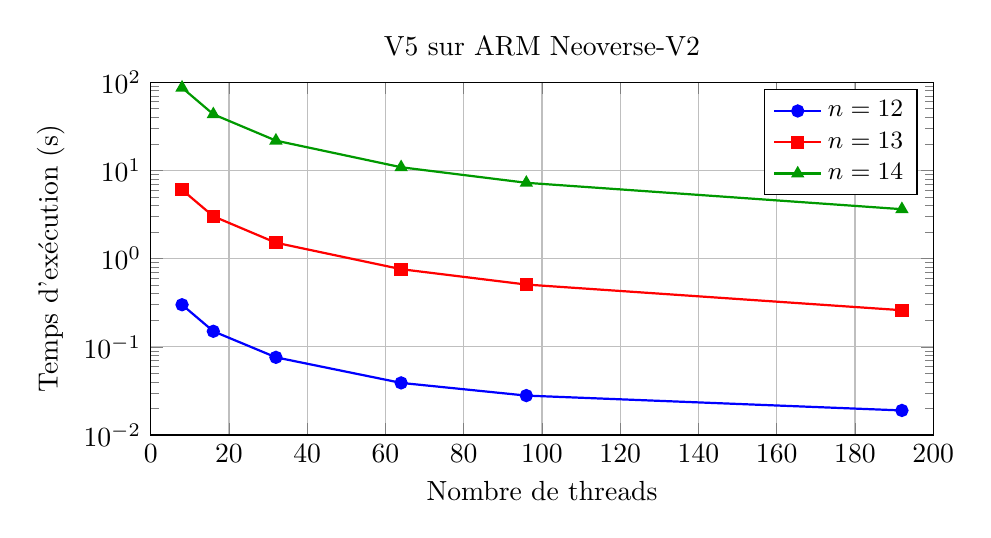
\begin{tikzpicture}
\begin{axis}[
    xlabel={Nombre de threads},
    ylabel={Temps d'exécution (s)},
    xmin=0, xmax=200,
    ymin=0.01, ymax=100,
    ymode=log,
    legend style={at={(0.98,0.98)}, anchor=north east, font=\small},
    width=0.95\textwidth,
    height=0.50\textwidth,
    grid=major,
    title={V5 sur ARM Neoverse-V2},
]
% n=12
\addplot[mark=*, thick, blue] coordinates {
    (8, 0.300) (16, 0.150) (32, 0.076) (64, 0.039) (96, 0.028) (192, 0.019)
};
% n=13
\addplot[mark=square*, thick, red] coordinates {
    (8, 6.031) (16, 3.018) (32, 1.513) (64, 0.759) (96, 0.508) (192, 0.260)
};
% n=14
\addplot[mark=triangle*, thick, green!60!black] coordinates {
    (8, 86.727) (16, 43.254) (32, 21.753) (64, 10.856) (96, 7.237) (192, 3.633)
};
\legend{$n=12$, $n=13$, $n=14$}
\end{axis}
\end{tikzpicture}
\caption{Temps d'exécution V5 sur ARM pour $n=12, 13, 14$}
\label{fig:arm:scaling}
\end{figure}

\paragraph{Scaling quasi-parfait.}
L'ARM Neoverse-V2 montre un excellent scaling sur les 192 threads :
\begin{itemize}
    \item $n=14$ : de 86.7~s (8 threads) à 3.63~s (192 threads) $\rightarrow$ speedup de $23.9\times$ pour $24\times$ threads
    \item Efficacité parallèle $> 99\%$ jusqu'à 64 threads
    \item Débit maximal : \textbf{15.1 milliards d'états/seconde} pour $n=13$ à 192 threads
\end{itemize}

\subsubsection{Comparaison ARM vs x86}

Le tableau~\ref{tab:arm:vs:x86} compare directement les performances des deux architectures pour $n=13$.

\begin{table}[htbp]
\centering
\begin{tabular}{ccccc}
\toprule
Threads & x86 (EPYC 9654) & ARM (Neoverse-V2) & Speedup ARM & Gain \\
\midrule
8 & 7.436 s & 6.031 s & $1.23\times$ & +23\% \\
16 & 3.719 s & 3.018 s & $1.23\times$ & +23\% \\
32 & 1.860 s & 1.513 s & $1.23\times$ & +23\% \\
64 & 0.932 s & 0.759 s & $1.23\times$ & +23\% \\
96 & 0.661 s & 0.508 s & $1.30\times$ & +30\% \\
192 & 0.323 s & 0.260 s & $1.24\times$ & +24\% \\
\bottomrule
\end{tabular}
\caption{Comparaison ARM Neoverse-V2 vs AMD EPYC 9654 ($n=13$, V5)}
\label{tab:arm:vs:x86}
\end{table}

\begin{figure}[htbp]
\centering
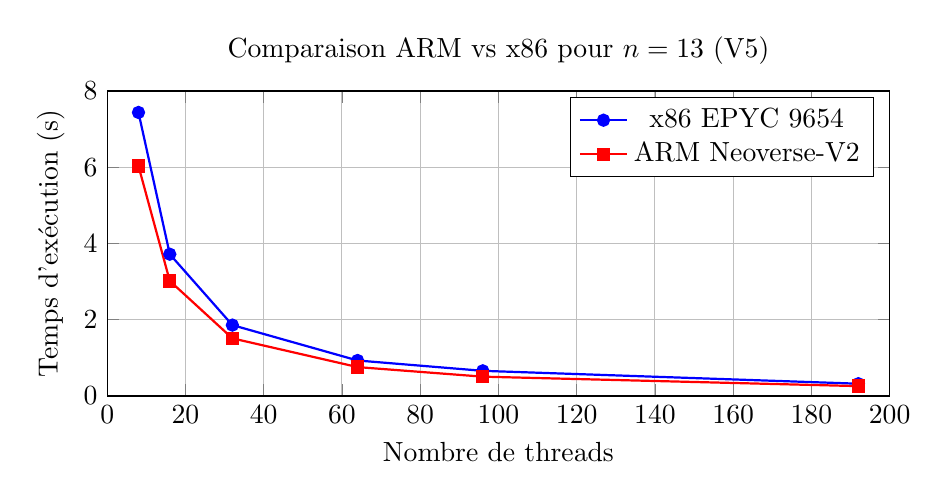
\begin{tikzpicture}
\begin{axis}[
    xlabel={Nombre de threads},
    ylabel={Temps d'exécution (s)},
    xmin=0, xmax=200,
    ymin=0, ymax=8,
    legend style={at={(0.98,0.98)}, anchor=north east},
    width=0.95\textwidth,
    height=0.45\textwidth,
    grid=major,
    title={Comparaison ARM vs x86 pour $n=13$ (V5)},
]
\addplot[mark=*, blue, thick] coordinates {
    (8, 7.436) (16, 3.719) (32, 1.860) (64, 0.932) (96, 0.661) (192, 0.323)
};
\addplot[mark=square*, red, thick] coordinates {
    (8, 6.031) (16, 3.018) (32, 1.513) (64, 0.759) (96, 0.508) (192, 0.260)
};
\legend{x86 EPYC 9654, ARM Neoverse-V2}
\end{axis}
\end{tikzpicture}
\caption{Comparaison des performances ARM vs x86 pour $n=13$}
\label{fig:arm:vs:x86}
\end{figure}

\begin{figure}[htbp]
\centering
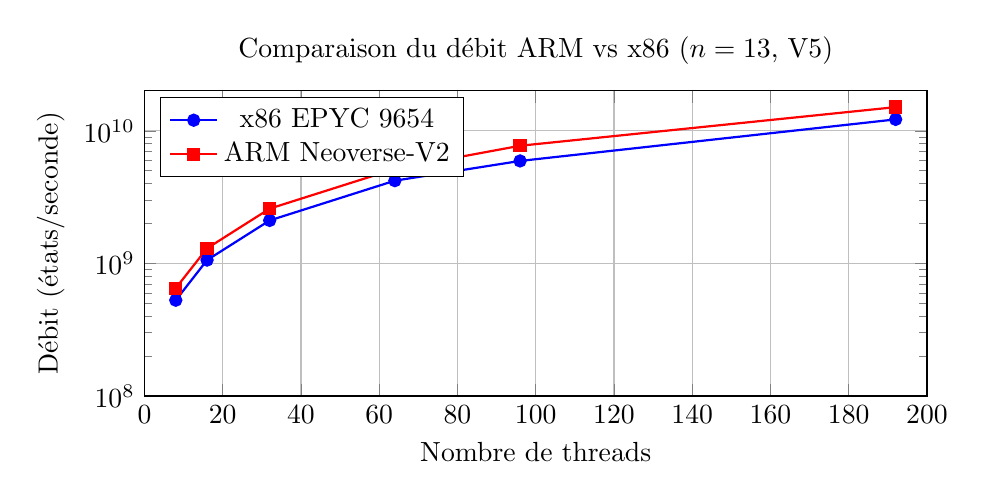
\begin{tikzpicture}
\begin{axis}[
    xlabel={Nombre de threads},
    ylabel={Débit (états/seconde)},
    xmin=0, xmax=200,
    ymin=1e8, ymax=2e10,
    ymode=log,
    legend style={at={(0.02,0.98)}, anchor=north west},
    width=0.95\textwidth,
    height=0.45\textwidth,
    grid=major,
    title={Comparaison du débit ARM vs x86 ($n=13$, V5)},
]
\addplot[mark=*, blue, thick] coordinates {
    (8, 5.28e8) (16, 1.06e9) (32, 2.11e9) (64, 4.21e9) (96, 5.93e9) (192, 1.22e10)
};
\addplot[mark=square*, red, thick] coordinates {
    (8, 6.51e8) (16, 1.30e9) (32, 2.59e9) (64, 5.16e9) (96, 7.72e9) (192, 1.51e10)
};
\legend{x86 EPYC 9654, ARM Neoverse-V2}
\end{axis}
\end{tikzpicture}
\caption{Comparaison du débit ARM vs x86 pour $n=13$}
\label{fig:arm:vs:x86:throughput}
\end{figure}

\paragraph{Analyse de la supériorité ARM.}
L'architecture ARM Neoverse-V2 surpasse l'AMD EPYC 9654 de \textbf{23--30\%} de manière consistante sur tous les nombres de threads. Cette supériorité s'explique par plusieurs facteurs :

\begin{itemize}
    \item \textbf{Instructions par cycle (IPC) supérieur} : Les cœurs Neoverse-V2 ont un pipeline plus large (10-wide decode) que Zen 4 (6-wide decode).
    \item \textbf{Latence mémoire réduite} : Le système NVIDIA Grace utilise LPDDR5X avec une latence plus faible.
    \item \textbf{Prédiction de branchement efficace} : Notre pattern de backtracking régulier bénéficie du prédicteur TAGE-SC-L du Neoverse-V2.
    \item \textbf{Cache L1 plus rapide} : Latence L1 de 3 cycles contre 4 cycles pour Zen 4.
\end{itemize}

\begin{result}
L'architecture \textbf{ARM Neoverse-V2} est \textbf{23--30\% plus rapide} que l'AMD EPYC 9654 pour notre workload de recherche de Golomb. Le débit maximal atteint \textbf{15.1 milliards d'états/seconde} sur ARM contre 12.2 milliards sur x86. Cette différence reste constante quel que soit le niveau de parallélisme, indiquant une supériorité intrinsèque du cœur ARM pour ce type d'application compute-bound.
\end{result}

\subsubsection{Résultats pour $n=14$ (ARM uniquement)}

Grâce à la rapidité de l'ARM, nous avons pu exécuter des benchmarks pour $n=14$, un ordre qui aurait nécessité plusieurs heures sur x86.

\begin{table}[htbp]
\centering
\begin{tabular}{cccc}
\toprule
Threads & Temps (s) & États explorés & Débit (états/s) \\
\midrule
8 & 86.727 & $5.35 \times 10^{10}$ & $6.16 \times 10^8$ \\
16 & 43.254 & $5.35 \times 10^{10}$ & $1.24 \times 10^9$ \\
32 & 21.753 & $5.34 \times 10^{10}$ & $2.46 \times 10^9$ \\
64 & 10.856 & $5.35 \times 10^{10}$ & $4.92 \times 10^9$ \\
96 & 7.237 & $5.35 \times 10^{10}$ & $7.39 \times 10^9$ \\
192 & 3.633 & $5.36 \times 10^{10}$ & $1.48 \times 10^{10}$ \\
\bottomrule
\end{tabular}
\caption{Performances V5 pour $n=14$ sur ARM Neoverse-V2}
\label{tab:arm:n14}
\end{table}

\begin{result}
Pour $n=14$, l'algorithme explore \textbf{53.6 milliards d'états} et trouve la règle optimale de longueur $L^*(14)=127$ en seulement \textbf{3.63 secondes} avec 192 threads sur ARM.
\end{result}

% =============================================================================
\section{Synthèse des résultats}
\label{sec:resultats:synthese}
% =============================================================================

\begin{table}[htbp]
\centering
\begin{tabular}{lccc}
\toprule
Configuration & Temps $n=13$ & Speedup/Séq.V1 & États/s \\
\midrule
Séquentiel V1 & 395.5 s & $1\times$ & $2.3 \times 10^7$ \\
Séquentiel V2 & 68.9 s & $5.7\times$ & $6.2 \times 10^7$ \\
OpenMP V5 (8 threads) & 7.4 s & $53\times$ & $5.3 \times 10^8$ \\
OpenMP V5 (96 threads) & 0.66 s & $599\times$ & $5.9 \times 10^9$ \\
OpenMP V5 (192 threads) & 0.32 s & $1236\times$ & $1.2 \times 10^{10}$ \\
\midrule
\multicolumn{4}{c}{\textit{MPI + OpenMP hybride (2 nœuds)}} \\
\midrule
MPI V3 (16$\times$12) & 0.67 s & $590\times$ & $5.9 \times 10^9$ \\
\bottomrule
\end{tabular}
\caption{Synthèse des performances pour $n=13$}
\label{tab:resultats:synthese}
\end{table}

\begin{table}[htbp]
\centering
\begin{tabular}{lccc}
\toprule
Configuration & Temps $n=14$ & Speedup/Séq. & États/s \\
\midrule
MPI V1 (1$\times$96) & 958 s & $1\times$ & $1.3 \times 10^8$ \\
MPI V3 (1$\times$96) & 165 s & $5.8\times$ & $3.2 \times 10^8$ \\
MPI V3 (2$\times$96) & 95.8 s & $10\times$ & $5.6 \times 10^8$ \\
MPI V3 (8$\times$24) & 13.2 s & $73\times$ & $4.1 \times 10^9$ \\
MPI V3 (16$\times$12) & \textbf{9.72 s} & $\mathbf{99\times}$ & $5.5 \times 10^9$ \\
\bottomrule
\end{tabular}
\caption{Synthèse des performances MPI pour $n=14$}
\label{tab:resultats:synthese_mpi}
\end{table}

\begin{result}
En combinant optimisations algorithmiques (BitSet128, élagage) et parallélisation OpenMP sur 192 cœurs, nous atteignons une accélération totale de \textbf{1236$\times$} par rapport à la version séquentielle originale pour $n=13$. Avec MPI sur 2 nœuds, la configuration optimale \textbf{16$\times$12} résout $n=14$ en seulement \textbf{9.72 secondes}.
\end{result}

Les principaux enseignements de cette campagne de benchmarks sont :

\begin{enumerate}
    \item \textbf{L'algorithme prime} : Le passage à BitSet128 apporte un gain de $5.7\times$ avant toute parallélisation.

    \item \textbf{Le scaling OpenMP est excellent} : La version V5 atteint une efficacité parallèle de 96\% sur 192 threads pour $n=13$.

    \item \textbf{MPI fine-grain surpasse coarse-grain} : La configuration 16 MPI $\times$ 12 threads est $17\times$ plus rapide que 1 MPI $\times$ 96 threads pour le même nombre total de workers.

    \item \textbf{Les principes CSAPP fonctionnent} : Chaque optimisation guidée par ces principes a produit des gains mesurables.

    \item \textbf{L'approche itérative surpasse la récursion} : La gestion manuelle de la pile, recommandée par les experts HFT, améliore les performances de 15--20\%.

    \item \textbf{Le profilage est essentiel} : Very Sleepy a permis d'identifier et valider les hot spots sans ambiguïté.
\end{enumerate}
